\section{Технический проект}
\subsection{Общая характеристика организации решения задачи}

Необходимо спроектировать и разработать сайт-форум для обсуждения на нём различных тем.


Веб-сайт — это комплекс взаимосвязанных электронных страниц, сгруппированных в разделы и доступных через уникальный интернет-адрес в форме www.имя\_сайта.ru. Каждая страница веб-сайта представляет собой текстовый документ, созданный с применением различных языков программирования, таких как HTML, CSS, JavaScript и другие.

\subsection{Обоснование выбора технологии проектирования}

На сегодняшний день информационный рынок, поставляющий программные решения в выбранной сфере, предлагает множество продуктов, позволяющих достигнуть поставленной цели – разработки web-сайта.

\subsubsection{Описание используемых технологий и языков программирования}

В процессе разработки web-сайта используются программные средства и языки программирования. Каждое программное средство и каждый язык программирования применяется для круга задач, при решении которых они необходимы.

\subsubsection{Язык программирования Python}

Python – это интерпретируемый, высокоуровневый язык программирования с динамической типизацией, который обеспечивает простоту в использовании, читаемость кода и эффективное взаимодействие с другими языками и системами. Основное предназначение данного языка – это создание серверной части веб-приложения, обеспечивая взаимодействие с веб-сервером. Это позволяет обрабатывать HTTP-запросы, управлять сессиями и осуществлять обработку данных от клиентов, а также взаимодействовать с базой данных.

\subsubsection{Язык программирования JavaScript}

\paragraph{Достоинства языка JavaScript}

JavaScript – это высокоуровневый, интерпретируемый язык программирования, который широко используется для создания интерактивных и динамичных веб-сайтов. Разработанный Netscape, JavaScript стал ключевым компонентом веб-технологий, позволяя веб-страницам взаимодействовать с пользователем, изменять содержимое и обеспечивать богатый пользовательский опыт. JavaScript используется для создания интерактивных элементов пользовательского интерфейса на веб-сайтах форумов. Это включает в себя динамическую подгрузку данных, анимации, обработку событий и обновление содержимого страницы без ее перезагрузки. JavaScript может обеспечивать валидацию данных, введенных пользователями в формах, перед отправкой на сервер. Также он применяется для асинхронного взаимодействия с сервером, например, для отправки комментариев, без необходимости перезагрузки всей страницы. JavaScript позволяет динамически обновлять содержимое форума в реальном времени. Это может включать в себя добавление новых тем, обновление сообщений, и другие изменения, которые пользователь может видеть без необходимости обновления всей страницы. JavaScript используется для взаимодействия с серверной частью, осуществляя запросы к API форума на Python. Это включает передачу данных между клиентом и сервером, а также обновление интерфейса в соответствии с полученными данными.

\paragraph{Недостатки языка Javascript}

JavaScript может вести себя по-разному в различных браузерах, что создает проблемы с кросс-браузерной совместимостью. Некоторые функции могут работать по-разному или вовсе отсутствовать в различных браузерах, что требует дополнительного тестирования и учета особенностей при разработке. JavaScript выполняется на стороне клиента, и поэтому пользователи могут иметь доступ к исходному коду и внести изменения. Это может создавать уязвимости безопасности, такие как внедрение вредоносного кода или модификация данных на стороне клиента. По соображениям безопасности JavaScript имеет ограниченный доступ к файловой системе клиентского устройства. Это может затруднить реализацию некоторых функций, таких как загрузка и сохранение файлов на стороне клиента. Средства отладки JavaScript в браузере могут быть менее мощными и удобными, чем средства отладки на сервере. Это может затруднить выявление и устранение ошибок в коде JavaScript. Обработка ошибок в JavaScript иногда может быть неочевидной из-за асинхронной природы языка. Это может затруднить выявление и отладку ошибок, особенно в сложных веб-приложениях.

\subsection{Диаграмма взаимодействия и схема обмена данными между представлениями}

Диаграмма взаимодействия описывает физическое представление системы и устанавливает связи между ее программными представлениями, включая исходный и исполняемый код. Она служит инструментом для определения архитектуры системы, выявляя зависимости между программными элементами. На диаграмме взаимодействия используются графические элементы, такие как представления, интерфейсы и их взаимосвязи.

На приведенной диаграмме, рисунок \ref{comp:image}, представлено взаимодействие в рамках проектируемой системы. Сервер, оснащенный операционной системой, содержит систему управления содержимым, включая базу данных и интерфейс. Также изображен клиентский компьютер с операционной системой, на котором установлен браузер. Данная диаграмма помогает визуализировать архитектурные компоненты и их взаимосвязи в физическом представлении системы.


\begin{figure}[ht]
\center{\includegraphics[width=1\linewidth]{comp}}
\caption{Диаграмма компонентов}
\label{comp:image}
\end{figure}

\vspace{+13mm} % чтобы убрать пустую строку, которая осталась после переноса рисунка на следующую страницу
\begin{figure}[ht]
	\center{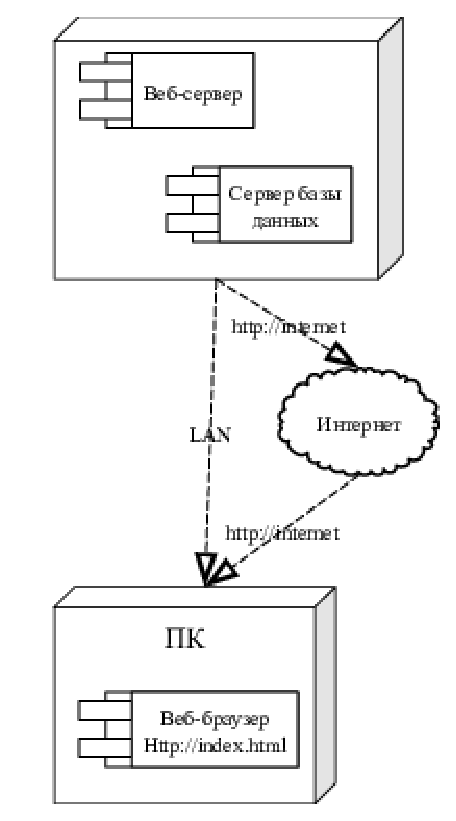
\includegraphics[width=0.57\linewidth]{place}}
	\caption{Диаграмма размещения}
	\label{place:image}
\end{figure}

Каждое представление должно быть активировано в контексте веб-страницы. В процессе вызова представления, данные передаются из веб-страницы в само представление.

Файл index.py представляет собой пример простого веб-приложения на Python, использующего фреймворк WSGI (Web Server Gateway Interface). В этом файле происходит импорт необходимых библиотек, классов и функций, таких как CGI, Waitress для веб-сервера, различные представления (views) и функции для работы с файлами и базой данных.



Словарь urls связывает URL-пути с соответствующими представлениями. Когда поступает запрос, код использует этот словарь для определения, какой обработчик использовать для конкретного URL. Основная функция app обрабатывает POST-запрос для загрузки файла, извлекает данные из формы, вставляет изображение в базу данных и возвращает ответ в формате JSON. Обработка GET-запроса осуществляется путем логики определения и вызова соответствующего представления, а также обработки статических файлов, установки MIME-типа и кодировки для ответа, установки заголовков ответа и возврата данных в ответе.

\subsection{Диаграмма размещения}

Диаграмма размещения (рис.~\ref{place:image}) отражает физические взаимосвязи между методами и представлениями.

Она является хорошим средством для показа маршрутов перемещения объектов и компонентов в распределенной системе.

\subsection{Содержание информационных блоков. Основные сущности}











Проанализировав требования, можно выделить три основных сущности:
\begin{itemize}
\item "<Пользователь">;
\item "<Сообщение">;
\item "<Тема">.
\end{itemize}

В состав сущности "<Сообщение"> можно включить атрибуты, представленные в таблице \ref{message:table}.

\begin{xltabular}{\textwidth}{|l|l|p{1.7cm}|X|}
	\caption{Атрибуты сущности "<Сообщение">\label{message:table}}\\ \hline
	\centrow Поле & \centrow Тип & \centrow Обяза\-тельное & \centrow Описание \\ \hline
	\thead{1} & \thead{2} & \centrow 3 & \centrow 4 \\ \hline
	\endfirsthead

	id\_message & Integer & true & Уникальный идентификатор сообщения \\ \hline 
	id\_user\_message & Integer & true & Уникальный идентификатор сообщения пользователя \\ \hline 
	topic\_id & Integer & true & Уникальный идентификатор темы, в которой написано сообщение \\ \hline 
	message\_text & String & true & Текст сообщения \\ \hline 
\end{xltabular}

В состав сущности "<Пользователь"> можно включить атрибуты, представленные в таблице \ref{user:table}.

\begin{xltabular}{\textwidth}{|l|lp{1.7cm}|X|}
	\caption{Атрибуты сущности "<Пользователь">\label{user:table}}\\ \hline
	\centrow Поле & \centrow Тип & \centrow Обяза\-тельное & \centrow Описание \\ \hline
	\thead{1} & \thead{2} & \centrow 3 & \centrow 4 \\ \hline
	\endfirsthead
	id\_user & Integer & true & Уникальный идентификатор пользователя \\ \hline 
	login & String & true & Имя пользователя \\ \hline 
	password & String & true & Пароль пользователя \\ \hline 
\end{xltabular}

В состав сущности "<Тема"> можно включить атрибуты, представленные в таблице \ref{topic:table}.

\begin{xltabular}{\textwidth}{|l|l|p{1.7cm}|X|}
	\caption{Атрибуты сущности "<Тема">\label{topic:table}}\\ \hline
	\centrow Поле & \centrow Тип & \centrow Обяза\-тельное & \centrow Описание \\ \hline
	\thead{1} & \thead{2} & \centrow 3 & \centrow 4 \\ \hline
	\endfirsthead
	id\_message & Integer & true & Уникальный идентификатор сообщения \\ \hline 
	id\_user\_message & Integer & true & Уникальный идентификатор сообщения пользователя \\ \hline 
	topic\_id & Integer & true & Уникальный идентификатор темы, в которой написано сообщение \\ \hline 
	message\_text & String & true & Текст сообщения \\ \hline 
\end{xltabular} 
